% options for packages loaded elsewhere
\PassOptionsToPackage{unicode=true}{hyperref}
\PassOptionsToPackage{hyphens}{url}
\PassOptionsToPackage{dvipsnames,svgnames*,x11names*}{xcolor}

% apa6 mode and class options
\documentclass[man,longtable,noextraspace,floatsintext]{apa6}

% for mode selection options
\usepackage{ifthen}

% setup mode ifs
\newif\ifmanmode
\newif\ifdocmode
\newif\ifjoumode
\ifthenelse{\equal{\string man}{\string man}}{
    \manmodetrue
}{
    \ifthenelse{\equal{\string man}{\string doc}}{
        \docmodetrue
    }{
        \ifthenelse{\equal{\string man}{\string jou}}{
            \joumodetrue
        }{
% None
}}}

% floatsintext

% other packages
\usepackage{lmodern}
\usepackage{amsmath,amssymb}
\usepackage{ifxetex,ifluatex}
\usepackage{fixltx2e} % provides \textsubscript

% handle different types of tex engines
% if pdftex
\ifnum 0\ifxetex 1\fi\ifluatex 1\fi=0
  \usepackage[T1]{fontenc}
  \usepackage[utf8]{inputenc}
  \usepackage{textcomp} % provides euro and other symbols
% if luatex or xelatex
\else
  \usepackage{unicode-math}
  \defaultfontfeatures{Ligatures=TeX,Scale=MatchLowercase}
\fi

% other language options
\usepackage[american]{babel}
\usepackage{csquotes}
\usepackage{microtype}

% disable microtype protrusion for tt fonts
\UseMicrotypeSet[protrusion]{basicmath}

\usepackage{graphicx,grffile}
% Scale images if necessary, so that they will not overflow the page
% margins by default, and it is still possible to overwrite the defaults
% using explicit options in \includegraphics[width, height, ...]{}
\makeatletter
\def\maxwidth{\ifdim\Gin@nat@width>\linewidth\linewidth\else\Gin@nat@width\fi}
\def\maxheight{\ifdim\Gin@nat@height>\textheight\textheight\else\Gin@nat@height\fi}
\makeatother
\setkeys{Gin}{width=\maxwidth,height=\maxheight,keepaspectratio}

\usepackage{booktabs}
\usepackage{caption}
\usepackage{subcaption}
\usepackage{xcolor}

% Pandoc stuff
\let\tightlist\relax % empty pandoc tight list command

% Hyperlinks and other metadata in pdf
\usepackage{hyperref}
\hypersetup{
            pdftitle={Writing an APA manuscript with Pandoc markdown},
            pdfauthor={Author 1, Author 2; Author 3},
            pdfkeywords={sublime text, vscode, pandoc, apa6},
            colorlinks=true,
            linkcolor=Blue,
            citecolor=Blue,
            urlcolor=Blue,
            breaklinks=true}
\urlstyle{same} % don't use monospace font for urls



\usepackage{color}
\usepackage{fancyvrb}
\newcommand{\VerbBar}{|}
\newcommand{\VERB}{\Verb[commandchars=\\\{\}]}
\DefineVerbatimEnvironment{Highlighting}{Verbatim}{commandchars=\\\{\}}
% Add ',fontsize=\small' for more characters per line
\newenvironment{Shaded}{}{}
\newcommand{\AlertTok}[1]{\textcolor[rgb]{1.00,0.00,0.00}{\textbf{#1}}}
\newcommand{\AnnotationTok}[1]{\textcolor[rgb]{0.38,0.63,0.69}{\textbf{\textit{#1}}}}
\newcommand{\AttributeTok}[1]{\textcolor[rgb]{0.49,0.56,0.16}{#1}}
\newcommand{\BaseNTok}[1]{\textcolor[rgb]{0.25,0.63,0.44}{#1}}
\newcommand{\BuiltInTok}[1]{#1}
\newcommand{\CharTok}[1]{\textcolor[rgb]{0.25,0.44,0.63}{#1}}
\newcommand{\CommentTok}[1]{\textcolor[rgb]{0.38,0.63,0.69}{\textit{#1}}}
\newcommand{\CommentVarTok}[1]{\textcolor[rgb]{0.38,0.63,0.69}{\textbf{\textit{#1}}}}
\newcommand{\ConstantTok}[1]{\textcolor[rgb]{0.53,0.00,0.00}{#1}}
\newcommand{\ControlFlowTok}[1]{\textcolor[rgb]{0.00,0.44,0.13}{\textbf{#1}}}
\newcommand{\DataTypeTok}[1]{\textcolor[rgb]{0.56,0.13,0.00}{#1}}
\newcommand{\DecValTok}[1]{\textcolor[rgb]{0.25,0.63,0.44}{#1}}
\newcommand{\DocumentationTok}[1]{\textcolor[rgb]{0.73,0.13,0.13}{\textit{#1}}}
\newcommand{\ErrorTok}[1]{\textcolor[rgb]{1.00,0.00,0.00}{\textbf{#1}}}
\newcommand{\ExtensionTok}[1]{#1}
\newcommand{\FloatTok}[1]{\textcolor[rgb]{0.25,0.63,0.44}{#1}}
\newcommand{\FunctionTok}[1]{\textcolor[rgb]{0.02,0.16,0.49}{#1}}
\newcommand{\ImportTok}[1]{#1}
\newcommand{\InformationTok}[1]{\textcolor[rgb]{0.38,0.63,0.69}{\textbf{\textit{#1}}}}
\newcommand{\KeywordTok}[1]{\textcolor[rgb]{0.00,0.44,0.13}{\textbf{#1}}}
\newcommand{\NormalTok}[1]{#1}
\newcommand{\OperatorTok}[1]{\textcolor[rgb]{0.40,0.40,0.40}{#1}}
\newcommand{\OtherTok}[1]{\textcolor[rgb]{0.00,0.44,0.13}{#1}}
\newcommand{\PreprocessorTok}[1]{\textcolor[rgb]{0.74,0.48,0.00}{#1}}
\newcommand{\RegionMarkerTok}[1]{#1}
\newcommand{\SpecialCharTok}[1]{\textcolor[rgb]{0.25,0.44,0.63}{#1}}
\newcommand{\SpecialStringTok}[1]{\textcolor[rgb]{0.73,0.40,0.53}{#1}}
\newcommand{\StringTok}[1]{\textcolor[rgb]{0.25,0.44,0.63}{#1}}
\newcommand{\VariableTok}[1]{\textcolor[rgb]{0.10,0.09,0.49}{#1}}
\newcommand{\VerbatimStringTok}[1]{\textcolor[rgb]{0.25,0.44,0.63}{#1}}
\newcommand{\WarningTok}[1]{\textcolor[rgb]{0.38,0.63,0.69}{\textbf{\textit{#1}}}}


% References
\usepackage[backend=biber,sortcites=true,style=apa,sorting=nyt,isbn=false,url=false]{biblatex}
\DeclareLanguageMapping{american}{american-apa}
\addbibresource{references.bib}

% Title page stuff
\title{Writing an APA manuscript with Pandoc markdown}
\shorttitle{Markdown to APA}
\twoauthors{Author 1, Author 2}{Author 3}
\twoaffiliations{Institute 1}{Institute 2}

\note{Last updated: \today}
\authornote{%
\noindent Correspondence:

Joseph M. Burling

Department of Psychology

6538 Franz Hall, UCLA

Los Angeles, CA 90095-1563

Email: jmburling@ucla.edu
}
% Abstract page
\abstract{%
This is just an example of using pandoc (with the help of some build
systems) to write in pandoc's markdown syntax for APA manuscripts. The
output will be rendered in APA 6 format according to some commands and
class options provided by the LaTeX \texttt{apa6} package. I also make
use of a few pandoc filters downloaded as python modules to get
cross-referencing to work. Lastly, I provide a .DOCX version of the
build system, though a lot may not translate and will require some
additional tweaking.
}
\keywords{sublime text, vscode, pandoc, apa6}

\ifdocmode
\usepackage{longtable}
\fi

\ifjoumode
% Journal specific commands may go here:
% two column long table. has to be done at the end
\usepackage{longtable}
\makeatletter
\let\oldlt\longtable
\let\endoldlt\endlongtable
\def\longtable{\@ifnextchar[\longtable@i \longtable@ii}
\def\longtable@i[#1]{%

\begin{figure}[btph]\onecolumn \begin{minipage}{0.5\textwidth} \oldlt[#1]}
\def\longtable@ii{\begin{figure}[btph]\onecolumn \begin{minipage}{0.5\textwidth} \oldlt}
\def\endlongtable{%
\endoldlt
\end{minipage}

\twocolumn
\end{figure}}
\makeatother
\fi

% table caption width
\makeatletter
\newcommand\LastLTentrywidth{1em}
\newlength\longtablewidth
\setlength{\longtablewidth}{1in}
\newcommand\getlongtablewidth{%
\begingroup
\ifcsname LT@\roman{LT@tables}\endcsname
\global\longtablewidth=0pt
\renewcommand\LT@entry[2]{\global\advance\longtablewidth by ##2\relax\gdef\LastLTentrywidth{##2}}%
\@nameuse{LT@\roman{LT@tables}}%
\fi
\endgroup}


\begin{document}
\maketitle

% pandoc-xnos: macro to create a caption without a prefix
\makeatletter
\def\LT@makenoprefixcaption#1#2#3{%
  \LT@mcol\LT@cols c{\hbox to\z@{\hss\parbox[t]\LTcapwidth{
    \sbox\@tempboxa{#1{}#3}
    \ifdim\wd\@tempboxa>\hsize
      #1{}#3
    \else
      \hbox to\hsize{\hfil\box\@tempboxa\hfil}%
    \fi
    \endgraf\vskip\baselineskip}
  \hss}}}
\makeatother

% pandoc-tablenos: save original macros
\makeatletter
\let\LT@oldmakecaption=\LT@makecaption
\let\oldthetable=\thetable
\let\oldtheHtable=\theHtable
\makeatother

% pandoc-tablenos: environment disables table caption prefixes
\makeatletter
\newcounter{tableno}
\newenvironment{no-prefix-table-caption}{
  \let\LT@makecaption=\LT@makenoprefixcaption
  \renewcommand\thetable{x.\thetableno}
  \renewcommand\theHtable{x.\thetableno}
  \stepcounter{tableno}
}{
  \let\thetable=\oldthetable
  \let\theHtable=\oldtheHtable
  \let\LT@makecaption=\LT@oldmakecaption
  \addtocounter{table}{-1}
}
\makeatother

\hypertarget{quick-pandoc-overview}{%
\section{Quick pandoc overview}\label{quick-pandoc-overview}}

The YAML metadata block is at the top of the document and take on
key-value pairs like so:

\begin{Shaded}
\begin{Highlighting}[]
\OtherTok{---}
\CommentTok{# string field with other characters should be quoted}
\FunctionTok{title:}\AttributeTok{ }\StringTok{"Some specials: Characters in the title?!?"}

\CommentTok{# toggle values}
\FunctionTok{twogroups:}\AttributeTok{ true}

\CommentTok{# nested fields with text}
\FunctionTok{joucommands:}
    \FunctionTok{leftheader:}\AttributeTok{ some ascii text}
    \FunctionTok{journal:}\AttributeTok{ other text}

\CommentTok{# lists}
\FunctionTok{bibliography:}
    \KeywordTok{-}\NormalTok{ references.bib}
    \KeywordTok{-}\NormalTok{ other_references.bib}

\CommentTok{# multiline text}
\FunctionTok{abstract:}\AttributeTok{ |}
\NormalTok{    lines go here}
\NormalTok{    and here.}
\OtherTok{---}
\end{Highlighting}
\end{Shaded}

Words go here, also here is a citation \autocite{someArticle}. According
to \textcite{anotherArticle}, something bad happened. See Figure
\ref{fig:myplot}. This is a bold statement\ldots{} \textbf{WOW!}, and
here's \_some \emph{emphasis for you} too. Sometimes you need some
typewrite-like font, like when writing code:
\texttt{my\_answer\ =\ 1\ +\ 1}. Other types you may need to write
blocks of code, like this:

\begin{Shaded}
\begin{Highlighting}[]
\KeywordTok{\textbackslash{}begin}\NormalTok{\{}\ExtensionTok{table}\NormalTok{\}}
\FunctionTok{\textbackslash{}centering}
\KeywordTok{\textbackslash{}begin}\NormalTok{\{}\ExtensionTok{tabular}\NormalTok{\}\{|l|l|\}}\FunctionTok{\textbackslash{}hline}
\NormalTok{Age }\OperatorTok{&}\NormalTok{ Frequency }\FunctionTok{\textbackslash{}\textbackslash{}} \FunctionTok{\textbackslash{}hline}
\NormalTok{18--25  }\OperatorTok{&}\NormalTok{ 15 }\FunctionTok{\textbackslash{}\textbackslash{}}
\NormalTok{26--35  }\OperatorTok{&}\NormalTok{ 33 }\FunctionTok{\textbackslash{}\textbackslash{}}
\NormalTok{36--45  }\OperatorTok{&}\NormalTok{ 22 }\FunctionTok{\textbackslash{}\textbackslash{}} \FunctionTok{\textbackslash{}hline}
\KeywordTok{\textbackslash{}end}\NormalTok{\{}\ExtensionTok{tabular}\NormalTok{\}}
\KeywordTok{\textbackslash{}end}\NormalTok{\{}\ExtensionTok{table}\NormalTok{\}}
\end{Highlighting}
\end{Shaded}

\begin{figure}
\centering
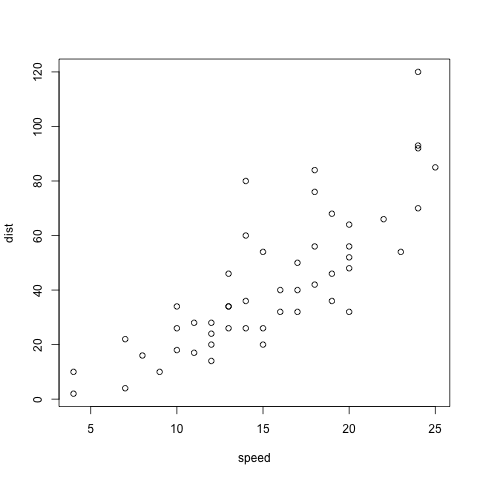
\includegraphics[width=3.333in,height=3.333in]{plot.png}
\caption{Your figure caption goes here.\label{fig:myplot}}
\end{figure}

See Table \ref{tbl:mytable} for an example on making tables using the
default extension. If tables are not referenced, then they are not given
table numbers and arranged with other tables. In APA man mode, Tables
are sent to the end of the document unless the following is used in the
YAML header at the top of this document:

\begin{Shaded}
\begin{Highlighting}[]
\FunctionTok{floatsintext:}\AttributeTok{ true}
\end{Highlighting}
\end{Shaded}

\begin{longtable}[]{@{}rllc@{}}
\caption{A table. \label{tbl:mytable}}\tabularnewline
\toprule
Right & Left & Default & Center\tabularnewline
\midrule
\endfirsthead
\toprule
Right & Left & Default & Center\tabularnewline
\midrule
\endhead
12 & 12 & 12 & 12\tabularnewline
123 & 123 & 123 & 123\tabularnewline
1 & 1 & 1 & 1\tabularnewline
\bottomrule
\end{longtable}

\begin{itemize}
\tightlist
\item
  This is another type of pandoc table (\ref{tbl:anotherone}). It should
  look the same.\footnote{Sometimes docx files will have tables that are
    squished. Autofit the document width to fix.}
\end{itemize}

\begin{longtable}[]{@{}rllc@{}}
\caption{Another one \label{tbl:anotherone}}\tabularnewline
\toprule
Right & Left & Default & Center\tabularnewline
\midrule
\endfirsthead
\toprule
Right & Left & Default & Center\tabularnewline
\midrule
\endhead
12 & 12 & 12 & 12\tabularnewline
123 & 123 & 123 & 123\tabularnewline
1 & 1 & 1 & 1\tabularnewline
\bottomrule
\end{longtable}

\newpage

\begin{no-prefix-table-caption}

\begin{longtable}[]{@{}lll@{}}
\caption{And another multi-line table which is more complicated to make.
It may require a pagebreak in two-column (jou) mode because pandoc uses
\texttt{longtable} which doesn't work in two-column mode. It has no
reference so it doesn't start with \enquote{Table x.} Some additional
latex hacks are added to the template to allow it to work (at the risk
of losing content or bleeding off the page. Blame pandoc for using
\texttt{longtable}).}\tabularnewline
\toprule
\begin{minipage}[b]{0.20\columnwidth}\raggedright
Fruit\strut
\end{minipage} & \begin{minipage}[b]{0.20\columnwidth}\raggedright
Price\strut
\end{minipage} & \begin{minipage}[b]{0.27\columnwidth}\raggedright
Advantages\strut
\end{minipage}\tabularnewline
\midrule
\endfirsthead
\toprule
\begin{minipage}[b]{0.20\columnwidth}\raggedright
Fruit\strut
\end{minipage} & \begin{minipage}[b]{0.20\columnwidth}\raggedright
Price\strut
\end{minipage} & \begin{minipage}[b]{0.27\columnwidth}\raggedright
Advantages\strut
\end{minipage}\tabularnewline
\midrule
\endhead
\begin{minipage}[t]{0.20\columnwidth}\raggedright
Bananas\strut
\end{minipage} & \begin{minipage}[t]{0.20\columnwidth}\raggedright
\$1.34\strut
\end{minipage} & \begin{minipage}[t]{0.27\columnwidth}\raggedright
\begin{itemize}
\tightlist
\item
  built-in wrapper
\item
  bright color
\end{itemize}\strut
\end{minipage}\tabularnewline
\begin{minipage}[t]{0.20\columnwidth}\raggedright
Oranges\strut
\end{minipage} & \begin{minipage}[t]{0.20\columnwidth}\raggedright
\$2.10\strut
\end{minipage} & \begin{minipage}[t]{0.27\columnwidth}\raggedright
\begin{itemize}
\tightlist
\item
  cures scurvy
\item
  tasty
\end{itemize}\strut
\end{minipage}\tabularnewline
\bottomrule
\end{longtable}

\end{no-prefix-table-caption}

Here's some raw latex code. It won't be recognized unless the output is
LaTeX/pdf and you have to proper parse-raw option set. It's the same
LaTeX code block from above rendered as an actual Table
\ref{tbl:rawtex}. The position may shift because it's a floating
environment.

\begin{table}
\centering
\caption{Using raw latex code}
\label{tbl:rawtex}
\begin{tabular}{|l|l|}\hline
Age & Frequency \\ \hline
18--25  & 15 \\
26--35  & 33 \\
36--45  & 22 \\ \hline
\end{tabular}
\end{table}

Checking rendering of Table \ref{tbl:tbllong}.

\begin{longtable}[]{@{}ccccccccc@{}}
\caption{Testing a longtable. \label{tbl:tbllong}}\tabularnewline
\toprule
id & sess & cond & rep & trial & age & demographic & gender &
maturation\tabularnewline
\midrule
\endfirsthead
\toprule
id & sess & cond & rep & trial & age & demographic & gender &
maturation\tabularnewline
\midrule
\endhead
S01 & -0.1706 & -B & -0.2317 & -0.3189 & -0.004132 & 1.103 & -m &
-pre\tabularnewline
S01 & -0.1706 & -A & -0.2317 & -0.2226 & -0.004132 & 1.103 & -m &
-pre\tabularnewline
S01 & -0.1706 & -C & -0.2317 & -0.1262 & -0.004132 & 1.103 & -m &
-pre\tabularnewline
S01 & -0.1706 & -C & 0.061 & -0.02987 & -0.004132 & 1.103 & -m &
-pre\tabularnewline
S01 & -0.1706 & -A & 0.061 & 0.06647 & -0.004132 & 1.103 & -m &
-pre\tabularnewline
S01 & -0.1706 & -A & 0.3537 & 0.1628 & -0.004132 & 1.103 & -m &
-pre\tabularnewline
S01 & -0.1706 & -C & 0.3537 & 0.2591 & -0.004132 & 1.103 & -m &
-pre\tabularnewline
S01 & -0.1706 & -B & 0.061 & 0.3555 & -0.004132 & 1.103 & -m &
-pre\tabularnewline
S01 & -0.1706 & -B & 0.3537 & 0.4518 & -0.004132 & 1.103 & -m &
-pre\tabularnewline
S01 & -0.1706 & -C & 0.6463 & 0.5482 & -0.004132 & 1.103 & -m &
-pre\tabularnewline
S01 & -0.1706 & -C & 0.939 & 0.6445 & -0.004132 & 1.103 & -m &
-pre\tabularnewline
S01 & -0.1706 & -B & 0.6463 & 0.7409 & -0.004132 & 1.103 & -m &
-pre\tabularnewline
S01 & -0.1706 & -A & 0.6463 & 0.8372 & -0.004132 & 1.103 & -m &
-pre\tabularnewline
S01 & -0.1706 & -B & 0.939 & 0.9335 & -0.004132 & 1.103 & -m &
-pre\tabularnewline
S01 & -0.1706 & -B & 1.232 & 1.03 & -0.004132 & 1.103 & -m &
-pre\tabularnewline
S01 & -0.1706 & -A & 0.939 & 1.126 & -0.004132 & 1.103 & -m &
-pre\tabularnewline
S01 & -0.1706 & -A & 1.232 & 1.223 & -0.004132 & 1.103 & -m &
-pre\tabularnewline
S01 & -0.1706 & -C & 1.232 & 1.319 & -0.004132 & 1.103 & -m &
-pre\tabularnewline
S02 & -0.1706 & -B & -0.2317 & -0.3189 & 0.01387 & 0.2929 & -m &
-pre\tabularnewline
S02 & -0.1706 & -A & -0.2317 & -0.2226 & 0.01387 & 0.2929 & -m &
-pre\tabularnewline
S02 & -0.1706 & -C & -0.2317 & -0.1262 & 0.01387 & 0.2929 & -m &
-pre\tabularnewline
S02 & -0.1706 & -A & 0.061 & -0.02987 & 0.01387 & 0.2929 & -m &
-pre\tabularnewline
S02 & -0.1706 & -A & 0.3537 & 0.06647 & 0.01387 & 0.2929 & -m &
-pre\tabularnewline
S02 & -0.1706 & -C & 0.061 & 0.1628 & 0.01387 & 0.2929 & -m &
-pre\tabularnewline
S02 & -0.1706 & -C & 0.3537 & 0.2591 & 0.01387 & 0.2929 & -m &
-pre\tabularnewline
S02 & -0.1706 & -A & 0.6463 & 0.3555 & 0.01387 & 0.2929 & -m &
-pre\tabularnewline
S02 & -0.1706 & -B & 0.061 & 0.4518 & 0.01387 & 0.2929 & -m &
-pre\tabularnewline
S02 & -0.1706 & -B & 0.3537 & 0.5482 & 0.01387 & 0.2929 & -m &
-pre\tabularnewline
S02 & -0.1706 & -B & 0.6463 & 0.6445 & 0.01387 & 0.2929 & -m &
-pre\tabularnewline
S02 & -0.1706 & -A & 0.939 & 0.7409 & 0.01387 & 0.2929 & -m &
-pre\tabularnewline
S02 & -0.1706 & -A & 1.232 & 0.8372 & 0.01387 & 0.2929 & -m &
-pre\tabularnewline
S02 & -0.1706 & -C & 0.6463 & 0.9335 & 0.01387 & 0.2929 & -m &
-pre\tabularnewline
S02 & -0.1706 & -C & 0.939 & 1.03 & 0.01387 & 0.2929 & -m &
-pre\tabularnewline
S02 & -0.1706 & -B & 0.939 & 1.126 & 0.01387 & 0.2929 & -m &
-pre\tabularnewline
S02 & -0.1706 & -C & 1.232 & 1.223 & 0.01387 & 0.2929 & -m &
-pre\tabularnewline
S02 & -0.1706 & -B & 1.232 & 1.319 & 0.01387 & 0.2929 & -m &
-pre\tabularnewline
S03 & -0.1706 & -A & -0.2317 & -0.3189 & -0.2321 & 1.464 & -m &
-pre\tabularnewline
S03 & -0.1706 & -B & -0.2317 & -0.2226 & -0.2321 & 1.464 & -m &
-pre\tabularnewline
S03 & -0.1706 & -A & 0.061 & -0.1262 & -0.2321 & 1.464 & -m &
-pre\tabularnewline
S03 & -0.1706 & -C & -0.2317 & -0.02987 & -0.2321 & 1.464 & -m &
-pre\tabularnewline
S03 & -0.1706 & -B & 0.061 & 0.06647 & -0.2321 & 1.464 & -m &
-pre\tabularnewline
S03 & -0.1706 & -A & 0.3537 & 0.1628 & -0.2321 & 1.464 & -m &
-pre\tabularnewline
S03 & -0.1706 & -A & 0.6463 & 0.2591 & -0.2321 & 1.464 & -m &
-pre\tabularnewline
S03 & -0.1706 & -B & 0.3537 & 0.3555 & -0.2321 & 1.464 & -m &
-pre\tabularnewline
S03 & -0.1706 & -C & 0.061 & 0.4518 & -0.2321 & 1.464 & -m &
-pre\tabularnewline
S03 & -0.1706 & -C & 0.3537 & 0.5482 & -0.2321 & 1.464 & -m &
-pre\tabularnewline
S03 & -0.1706 & -A & 0.939 & 0.6445 & -0.2321 & 1.464 & -m &
-pre\tabularnewline
S03 & -0.1706 & -C & 0.6463 & 0.7409 & -0.2321 & 1.464 & -m &
-pre\tabularnewline
S03 & -0.1706 & -B & 0.6463 & 0.8372 & -0.2321 & 1.464 & -m &
-pre\tabularnewline
S03 & -0.1706 & -C & 0.939 & 0.9335 & -0.2321 & 1.464 & -m &
-pre\tabularnewline
\bottomrule
\end{longtable}

\begin{itemize}
\item
  Here's an example of inline LaTeX math, \(p=.0499\).
\item
  Here's a an example of using LaTeX syntax for displaying equations.
\end{itemize}

\[
\hat{y} = \beta_0 + \beta_1 x
\]

Pandoc doesn't know how to make inline headings when converting to Word.
If you put the cursor at the end of the heading, press Ctrl+Alt+Enter
and it will move it down.

\hypertarget{subsection-heading}{%
\subsection{Subsection heading}\label{subsection-heading}}

Lorem ipsum dolor sit amet, consectetur adipiscing elit. Nulla et magna
vitae ipsum rhoncus congue eu vehicula sem. Vestibulum venenatis mauris
ac urna porta placerat. Ut ante neque, malesuada ut lobortis
ullamcorper, consectetur vitae ipsum. Morbi sodales, justo eu pretium
venenatis, sem libero dapibus sem, at molestie lectus felis ut nunc.
Praesent ultrices sagittis porta. Curabitur diam elit, lacinia nec
egestas sit amet, convallis a felis. Praesent dictum nec mauris quis
molestie. Proin ullamcorper, mauris sed molestie aliquet, nisi sapien
tempor risus, quis congue sapien turpis et justo. Suspendisse potenti.

Duis viverra aliquet metus, eget aliquam tellus mollis imperdiet. Lorem
ipsum dolor sit amet, consectetur adipiscing elit. Nulla et magna vitae
ipsum rhoncus congue eu vehicula sem. Vestibulum venenatis mauris ac
urna porta placerat. Ut ante neque, malesuada ut lobortis ullamcorper,
consectetur vitae ipsum. Morbi sodales, justo eu pretium venenatis, sem
libero dapibus sem, at molestie lectus felis ut nunc. Praesent ultrices
sagittis porta. Curabitur diam elit, lacinia nec egestas sit amet,
convallis a felis.

\hypertarget{subsubsection-heading}{%
\subsubsection{Subsubsection heading}\label{subsubsection-heading}}

Nullam nec est ut mauris eleifend pulvinar ac in nisl. In eleifend,
velit et rhoncus pretium, justo lectus viverra enim, nec feugiat ante
mauris vitae magna. Lorem ipsum dolor sit amet, consectetur adipiscing
elit. Morbi felis nulla, iaculis dapibus sapien quis, pretium laoreet
est. Mauris vel sapien tempor, dapibus ipsum sit amet, sagittis tellus.
Aliquam ipsum metus, ultricies eleifend dolor nec, ultricies mollis
sapien. Integer placerat ante condimentum sagittis elementum. Fusce
aliquam, libero a iaculis eleifend, ipsum ante tincidunt ante, ut
bibendum dolor risus ut nibh. Sed fermentum tellus id ligula sodales, ut
condimentum tortor tempus. Phasellus suscipit dapibus est sed
consectetur.

Nullam nec est ut mauris eleifend pulvinar ac in nisl. In eleifend,
velit et rhoncus pretium, justo lectus viverra enim, nec feugiat ante
mauris vitae magna. Lorem ipsum dolor sit amet, consectetur adipiscing
elit. Morbi felis nulla, iaculis dapibus sapien quis, pretium laoreet
est. Mauris vel sapien tempor, dapibus ipsum sit amet, sagittis tellus.
Aliquam ipsum metus, ultricies eleifend dolor nec, ultricies mollis
sapien. Integer placerat ante condimentum sagittis elementum. Fusce
aliquam, libero a iaculis eleifend, ipsum ante tincidunt ante, ut
bibendum dolor risus ut nibh. Sed fermentum tellus id ligula sodales, ut
condimentum tortor tempus. Phasellus suscipit dapibus est sed
consectetur.

\hypertarget{paragraph-heading}{%
\paragraph{Paragraph heading}\label{paragraph-heading}}

Lorem ipsum dolor sit amet, consectetur adipiscing elit. Nulla et magna
vitae ipsum rhoncus congue eu vehicula sem. Vestibulum venenatis mauris
ac urna porta placerat. Ut ante neque, malesuada ut lobortis
ullamcorper, consectetur vitae ipsum. Morbi sodales, justo eu pretium
venenatis, sem libero dapibus sem, at molestie lectus felis ut nunc.
Praesent ultrices sagittis porta. Curabitur diam elit, lacinia nec
egestas sit amet, convallis a felis. Praesent dictum nec mauris quis
molestie. Proin ullamcorper, mauris sed molestie aliquet, nisi sapien
tempor risus, quis congue sapien turpis et justo. Suspendisse potenti.
Duis viverra aliquet metus, eget aliquam tellus mollis imperdiet.

\hypertarget{subparagraph-heading}{%
\subparagraph{Subparagraph heading}\label{subparagraph-heading}}

Lorem ipsum dolor sit amet, consectetur adipiscing elit. Nulla et magna
vitae ipsum rhoncus congue eu vehicula sem. Vestibulum venenatis mauris
ac urna porta placerat. Ut ante neque, malesuada ut lobortis
ullamcorper, consectetur vitae ipsum. Morbi sodales, justo eu pretium
venenatis, sem libero dapibus sem, at molestie lectus felis ut nunc.
Praesent ultrices sagittis porta. Curabitur diam elit, lacinia nec
egestas sit amet, convallis a felis. Praesent dictum nec mauris quis
molestie. Proin ullamcorper, mauris sed molestie aliquet, nisi sapien
tempor risus, quis congue sapien turpis et justo. Suspendisse potenti.
Duis viverra aliquet metus, eget aliquam tellus mollis imperdiet.

Getting silly with the amount of subheadings

Lorem ipsum dolor sit amet, consectetur adipiscing elit. Nulla et magna
vitae ipsum rhoncus congue eu vehicula sem. Vestibulum venenatis mauris
ac urna porta placerat. Ut ante neque, malesuada ut lobortis
ullamcorper, consectetur vitae ipsum. Morbi sodales, justo eu pretium
venenatis, sem libero dapibus sem, at molestie lectus felis ut nunc.
Praesent ultrices sagittis porta. Curabitur diam elit, lacinia nec
egestas sit amet, convallis a felis. Praesent dictum nec mauris quis
molestie. Proin ullamcorper, mauris sed molestie aliquet, nisi sapien
tempor risus, quis congue sapien turpis et justo. Suspendisse potenti.
Duis viverra aliquet metus, eget aliquam tellus mollis imperdiet.

Nullam nec est ut mauris eleifend pulvinar ac in nisl. In eleifend,
velit et rhoncus pretium, justo lectus viverra enim, nec feugiat ante
mauris vitae magna. Lorem ipsum dolor sit amet, consectetur adipiscing
elit. Morbi felis nulla, iaculis dapibus sapien quis, pretium laoreet
est. Mauris vel sapien tempor, dapibus ipsum sit amet, sagittis tellus.
Aliquam ipsum metus, ultricies eleifend dolor nec, ultricies mollis
sapien. Integer placerat ante condimentum sagittis elementum. Fusce
aliquam, libero a iaculis eleifend, ipsum ante tincidunt ante, ut
bibendum dolor risus ut nibh. Sed fermentum tellus id ligula sodales, ut
condimentum tortor tempus. Phasellus suscipit dapibus est sed
consectetur.

Heading 7

Lorem ipsum dolor sit amet, consectetur adipiscing elit.

Heading 8

Lorem ipsum dolor sit amet, consectetur adipiscing elit.

\newpage

\printbibliography[title=References]



\end{document}
